\documentclass[11pt]{article}
\usepackage[margin=1in]{geometry}
\usepackage{amsmath,amssymb,booktabs,graphicx,hyperref,longtable,enumitem,xcolor,float}
\usepackage{xr}
\externaldocument{paper_nips_SUBMISSION_v11.8}
\graphicspath{{figures/}}
\title{Supplementary Information \\ \large \textbf{PGOB: Behavior-only parameter generation for whole-organism biophysical simulators across worm and fly} \\ \large Extended Methods, Extended Results, Negative-Results Ledger, Reproducibility, 3 non-invasive deployment modes across worm and fly simulators.}
\author{Chenxi He, University of Cambridge \\ \texttt{ch2067@cam.ac.uk}}

\begin{document}
\maketitle
\tableofcontents

This SI accompanies the main paper and provides extended methods, extended results, the consolidated negative-results ledger, and reproducibility details.

%==========================================================
\section{Hardware and Reproducibility (S1)}
\label{si:hardware}
%==========================================================

\textbf{Compute.} Cloud A40 GPU instances; RTX 4090D and RTX 3080 Ti secondary. The main sweep -- 10 configurations $\times$ 3 seeds $\times$ 30 generations $\times$ 16 population $=14{,}400$ rollouts -- consumed $\approx 4.8\times 10^4$ rollout-seconds ($\approx 27$ wall-hours). Cumulative compute: $\approx 307$ CPU-days (BAAIWorm 142, flybody 88, modWorm 41, FlyGym 36). Every reported result is reproducible from \texttt{python run\_calibration.py --sim \{worm,modworm,fly,flygym\} --scale s --seed k --opt cmaes\_sep}.

\subsection{Cohort-size notation (S1.1)}
$n{=}5,10$ = random SPSA seeds (weight-corruption and F1 ablation contexts); $n{=}4,40,160$ = starting conditions (held-out OOD context); $n{=}43$ = held-out mutant strains (Yemini prospective); $n{=}15$ = BAAIWorm ablation-type rank test; $n{=}5$/level ($30$ cells) = weight-corruption sweep; $N{=}200$ = OWMD-Schafer worms; $B{=}1000$ = bootstrap resamples. All ambiguous in-text occurrences are tagged with explicit unit names.

\textbf{Per-simulator hyperparameters.}

\begin{table}[H]\centering\small
\begin{tabular}{lccc}\toprule
Item & BAAIWorm & flybody & modWorm \\\midrule
Param dim & 5 (global scales) / $\approx$5k (full5 per-element) & 515 & 30/50 \\
Search-space transform & linear $[0.5,2]$ (scales); per-element (full5) & log-space mult. & linear \\
Integrator / $dt$ & RK4 1ms & MuJoCo 0.1ms & implicit-Euler 0.5ms \\
Output rate & 30 Hz & 10 kHz & 25 Hz \\
Rollout length & 10 s & 5 s & 40 s \\
Optimiser & SPSA + CMA & CMA-ES sep & CMA-ES sep \\
Population $\lambda$ & 8 / 8 & 16 & 16 \\
Generations & 30 & 30 & 30 \\
$\sigma_0$ & 0.05 & 0.05 log-space & 0.05 \\
Multi-cond avg $C$ & $[8,16]$ & 8 snippets & 8 seeds \\
\bottomrule
\end{tabular}
\caption{Per-simulator consolidated hyperparameter reference.}
\end{table}

%==========================================================
\section{Negative Results and Limitations (S2)}
\label{si:negatives}
%==========================================================

\subsection{Negative-Results Ledger -- Consolidated Single-Location Reference (S2.0)}
\noindent\textbf{Why this table exists.} This ledger consolidates every negative result, bounded-scope statement, and limitation from the submission into one place, so a reader can review all limitations together rather than tracking them across sections. Every row carries a back-pointer to the section where the underlying analysis lives; the main-text Scope-and-limitations box (\S\ref{sec:intro}) is the summary of this ledger.

\begin{table}[H]\centering\footnotesize
\caption{\textbf{Consolidated negative-results ledger.} Entries spanning bounded-scope statements, control results (S2.9), and per-channel residuals.}
\label{tab:ledger}
\begin{tabular}{p{0.30\textwidth} p{0.45\textwidth} p{0.16\textwidth}}\toprule
Finding & Caveat / scope & Section \\\midrule
4-config non-scalar loss falsification & Aggregate baseline dominates; no tested loss configuration dominates. & S2.5 \\
F1 ablation neural control ($10$ paired seeds, $n{=}20$ runs) & Pre-registered NULL (Wilcoxon $p{=}0.734$, $d{=}0.14$). Pure-trajectory loss is not outperformed by neural-augmented loss -- positive for the framework. (S4.4.1) & S2.9 \\
modWorm three-segment & Eigenworm-variance channels unmovable even at expert arm: substrate ceiling, $-9.9\%$ aggregate (S4.18). & S4.18 \\
flybody $W_1$ three-segment & Pre-registered null result: all three arms within $<1.5\%$ ($13.254/13.454/13.348$); \texttt{walk\_imitation} MoCap controller dominates trajectory, init signal carried in loss space ($9.3\times$), not $W_1$ (S4.18). & S4.18 \\
Extended-budget hybrid fine-tune & Useful but mild ($-1.1\%$/$-5.5\%$/$-2.0\%$ held-out dips): warm-start near irreducible sim$\leftrightarrow$real floor (S4.23). & S4.23 \\
flybody default-vs-PGOB & $0/9$ significant ($N{=}45$/arm): good default $\Rightarrow$ correct NULL (S4.21). & S4.21 \\
41-experiment GAN-as-loss collapse & Val-loss $\geq 2\times$ regression across 5 D-architectures. & S2.10 \\
Same-species parameter-prior transfer & Genuine same-species rescue (BAAIWorm$\to$modWorm $N{=}16$, flybody self-prior $9.3\times$); transfer demonstrated between two simulators of the same species only. & S4.5 \\
flybody FULL-split parity & TEST split $9/10$ closer at $+1.75\%$; FULL split caveated. & S4.2 \\
Loss-family invariance & Reported as an observation in the operational sense, not a Fisher / Cram\'er--Rao claim. & S4.7 \\
\bottomrule
\end{tabular}
\end{table}

\subsection{Non-scalar loss falsification (S2.5)}
4-configuration loss-design falsification on BAAIWorm; aggregate baseline dominates 3/5 metrics; no tested configuration dominates.

\subsection{F1 ablation control (S2.9)}
The neural-ablation control ($10$ paired seeds, $n{=}20$ runs) returns a pre-registered NULL (Wilcoxon $p{=}0.734$, $d{=}0.14$); pure-trajectory loss is not outperformed by neural-augmented loss. Full statistics in S4.4.1.

\subsection{41-experiment GAN-as-loss negative (S2.10)}
All 41 collapse: val-loss regresses $\geq 2\times$ while D-loss drops $<0.01$. A multi-behaviour discriminator on closed-loop FlyGym extends the same negative: a discriminator trained jointly on four behaviours does not outperform single-task discriminators ($\Delta{\approx}-0.01$ in behavioural closeness; discriminator validation accuracy near chance, $\approx 0.43$--$0.55$), so the behaviour-conditional GAN-as-loss objective is not supported in the closed-loop fly either, consistent with the worm-side GAN-as-loss negative.

%==========================================================
\section{Extended Methods (S3)}
\label{si:methods}
%==========================================================

\subsection{Universal 23-metric evaluator (S3.1)}
\begin{table}[H]\centering\small
\begin{tabular}{rlcccl}\toprule
\# & Metric & Definition & Worm & Fly & Function \\\midrule
1 & zigzag & running $\sum|\Delta h|$ over 1-s window & \checkmark & \checkmark & \texttt{\_zigzag} \\
2 & mean\_speed & $\langle\|\dot p_t\|\rangle$ & \checkmark & \checkmark & \texttt{\_mean\_speed} \\
3 & reversal\_frequency & $\#\{t: \dot p_t \cdot \hat h_t < 0\}/T$ & \checkmark & $\times$ & \texttt{\_reversal\_freq} \\
4 & wave\_amplitude & tangent-angle PC1 envelope max-min & \checkmark & $\times$ & \texttt{\_wave\_amp} \\
5 & speed\_std & $\text{std}(\|\dot p_t\|)$ & \checkmark & \checkmark & \texttt{\_speed\_std} \\
6 & chemotaxis\_index & $\langle\hat h_t \cdot \nabla c_t\rangle$ & \checkmark & $\times$ & \texttt{\_chemotaxis} \\
7 & distance\_to\_food & $\|p_T - p_{\rm food}\|$ & \checkmark & $\times$ & \texttt{\_dist\_food} \\
8 & steering & mean $|\dot{\hat h}_t|$ & \checkmark & \checkmark & \texttt{\_steering} \\
9 & turning\_rate & $\#\{t: \dot{\hat h}_t > 200{\rm deg/s}\}/T$ & \checkmark & \checkmark & \texttt{\_turn\_rate} \\
10 & body\_wave\_freq & dominant FFT freq & \checkmark & $\times$ & \texttt{\_wave\_freq} \\
11 & dorsal\_ventral\_corr & corr(d-arc, v-arc) & \checkmark & $\times$ & \texttt{\_dv\_corr} \\
12 & leg\_alternation & 6-leg phase-diff variance & $\times$ & \checkmark & \texttt{\_leg\_alt} \\
13 & MSD & slope & \checkmark & \checkmark & \texttt{\_msd} \\
14 & tortuosity & path / displacement & \checkmark & \checkmark & \texttt{\_tortuosity} \\
15 & path\_length & $\sum\|\Delta p_t\|$ & \checkmark & \checkmark & \texttt{\_path\_len} \\
16 & mean\_displacement & $\|p_T-p_0\|$ & \checkmark & \checkmark & \texttt{\_mean\_disp} \\
17 & mean\_acceleration & $\langle\|\ddot p_t\|\rangle$ & \checkmark & \checkmark & \texttt{\_mean\_acc} \\
18 & jerk & $\langle\|\dddot p_t\|\rangle$ & \checkmark & \checkmark & \texttt{\_jerk} \\
19 & heading\_variance & var$(\hat h_t)$ & \checkmark & \checkmark & \texttt{\_heading\_var} \\
20--23 & eigen\_e1--e4 & Stephens-2008 PC amplitudes & \checkmark & $\times$ & \texttt{\_eigen} \\\bottomrule
\end{tabular}
\caption{The v1 production code path emits 14; the v2 extension restores 9 missing scalars as pure-trajectory functions.}
\end{table}

\subsection{Three-distance computation (S3.2)}
$D_1 = \mathrm{d}_z(f_{\hat\theta},\{f_{\theta_{\rm GT}}\})$, $D_2 = \frac{1}{N}\sum_i \mathrm{d}_z(x^{(i)},\{x^{(j)}\}_{j\ne i})$, $D_3 = \mathrm{d}_z(f_{\theta_{\rm GT}},\{x^{(i)}\})$. Both naive z and median/MAD robust z reported.

\subsection{Eigenworm cross-validation (S3.3)}
Tangent-angle PCA cross-validated against OWMD Tierpsy on $n{=}40$ worms $\times$ 4 PC amplitudes: Pearson $r{=}0.987$.

\subsection{Same-species prior-transfer protocol (S3.5)}
The same-species parameter-prior transfer (S4.5/S4.6) derives a per-biophysical-class coefficient-of-variation prior from a source simulator and applies it as the per-dimension CMA-ES step size ($\sigma_0$) when generating on a different simulator of the same species. Each generation is one CMA-ES sep run (30 gen, $\lambda{=}16$); arms (random / cross-sim prior / own default) differ only in the prior used to seed $\sigma$, and are compared on a disjoint held-out test split. The cross-scale optimiser comparison fixes the simulator and the ground-truth $\theta^{*}$ and varies only the perturbation scale and optimiser (CMA-ES / DE / NES) at a matched eval budget.

%==========================================================
\section{Extended Results (S4)}
\label{si:results}
%==========================================================

\subsection{BAAIWorm three-distance hierarchy (S4.1)}
\begin{table}[H]\centering\small
\caption{Three-distance hierarchy, BAAIWorm full5 $\to$ OWMD-N2 ($N{=}200$). The \textbf{robust (MAD) $z$} estimator is the canonical one used throughout the main text ($D_1{=}0.71$, $D_2{=}1.98$, $D_3{=}21.82$); the other rows are sensitivity checks under alternative estimators. The strict $D_1{<}D_2{\ll}D_3$ hierarchy holds under the canonical estimator and the naive estimator; under the alternative $5$-active-feature cross-validated $D_2$ estimator the real$\leftrightarrow$real reference contracts to $0.393$ so $D_1$ no longer falls below it, but $D_1{<}D_3$ still holds by $30\times$. We report the robust estimator as canonical because the cross-validated $D_2$ uses a held-out feature subset that under-counts genuine inter-individual spread.}
\begin{tabular}{lcccc}\toprule
estimator & $D_1$ & $D_2$ & $D_3$ & hierarchy \\\midrule
\textbf{robust (MAD), canonical} & \textbf{0.713} & \textbf{1.976} & \textbf{21.82} & $D_1<D_2<D_3$ \\
naive & 0.500 & 1.780 & 26.47 & $D_1<D_2<D_3$ \\
trimmed 5\% & --- & 2.366 & 30.32 & $D_2<D_3$ \\
5-active-feature CV (sensitivity) & 0.713 & 0.393 & 21.82 & $D_1<D_3$ ($30\times$); marginal vs.\ $D_2$ \\\bottomrule
\end{tabular}
\end{table}
Bootstrap $B{=}1000$ on OWMD-N2 under the canonical robust estimator: $D_1<D_2<D_3$ in $1000/1000$.

\subsection{Drosophila parity (S4.2)}
\textbf{flybody walking TEST split}: $9/10$ closer at $+1.75\%$ ($60$ train / $20$ val / $20$ holdout). FULL-split caveat: default already strong; PGOB room marginal under FULL split. \textbf{Flight wing-beat} $227.92\pm 5.59$ Hz. \textbf{FlyGym 5-behaviour}: $5/5$ inside biological CV. \textbf{Adhesion phenotype}: 3-of-3 / 0-of-3 split.

\subsection{Yemini 43-strain (S4.3)}
\textbf{In-sample reference}: $\bar\rho{=}0.558$, median $0.400$, $43/43$ positive. \textbf{LOSO} (main-text Table~\ref{tab:loso_summary}): mean-train $0.684$, median-train $0.628$, strain-shuffle $0.527$.

\textbf{Pre-registered full $23$-feature LOSO robustness.} To confirm the $4$-feature headline is not an artefact of post-hoc feature selection, we re-ran the leave-one-strain-out test on the \emph{pre-registered full $23$-feature} set (fixed before scoring; the $4$ active features are a strict subset). Mean-training-delta Spearman $\bar\rho{=}0.525$ (median $0.585$, SD $0.211$) vs.\ strain-shuffle null $\bar\rho_0{=}0.338$ (median $0.352$, SD $0.114$), giving $\Delta{=}{+}0.187$ with $27/28$ strains $\rho{>}0$. The mutant-prediction signal is therefore preserved across the full deposited metric space, and the $4$- and $23$-feature analyses are mutually consistent. \emph{Caveat}: this full-feature LOSO ran on the $28$ mutant strains whose Yemini HDF5 features were retrievable from source ($14$ of the $43$ strain folders lacked retrievable feature data); it is a $28$-strain confirmation rather than the full $43$-strain panel. Mutant differential $N{=}12$ protocol: strain-specific 5/4/4 deviations.

\subsection{BAAIWorm $30$-cell weight-corruption (S4.4)}
\begin{longtable}{l l r r r r r}\toprule
Level & Seed & $L_0$ & $L_{\rm final}$ & $L_{\rm rec.\ clean}$ & $\Delta/L_0$ & elapsed (s) \\\midrule\endhead
L0 clean & 0 & 0.12479 & 0.06334 & 0.06334 & $-49.2\%$ & 7511 \\
L0 clean & 1 & 0.12479 & 0.08568 & 0.08568 & $-31.3\%$ & 7307 \\
L0 clean & 2 & 0.12479 & 0.06058 & 0.06058 & $-51.5\%$ & 7517 \\
L0 clean & 3 & 0.12479 & 0.06466 & 0.06466 & $-48.2\%$ & 7457 \\
L0 clean & 4 & 0.12479 & 0.07360 & 0.07360 & $-41.0\%$ & 7379 \\
L1 $5\%$ Gauss & 0 & 0.11695 & 0.07723 & 0.11474 & $-34.0\%$ & 7551 \\
L1 $5\%$ Gauss & 1 & 0.12690 & 0.04444 & 0.14148 & $-65.0\%$ & 7449 \\
L1 $5\%$ Gauss & 2 & 0.07772 & 0.05069 & 0.12691 & $-34.8\%$ & 7397 \\
L1 $5\%$ Gauss & 3 & 0.13131 & 0.05777 & 0.14815 & $-56.0\%$ & 7309 \\
L1 $5\%$ Gauss & 4 & 0.05706 & 0.04399 & 0.11078 & $-22.9\%$ & 7384 \\
L2 $20\%$ Gauss & 0 & 0.15749 & 0.14383 & 0.13439 & $-8.7\%$ & 7355 \\
L2 $20\%$ Gauss & 1 & 0.25744 & 0.21711 & 0.09803 & $-15.7\%$ & 7279 \\
L2 $20\%$ Gauss & 2 & 0.12516 & 0.07092 & 0.15990 & $-43.3\%$ & 7372 \\
L2 $20\%$ Gauss & 3 & 0.04760 & 0.04610 & 0.17732 & $-3.2\%$ & 7658 \\
L2 $20\%$ Gauss & 4 & 0.08930 & 0.04695 & 0.11239 & $-47.4\%$ & 7545 \\
L3 $50\%$ Gauss & 0 & 0.25733 & 0.20162 & 0.08917 & $-21.6\%$ & 7280 \\
L3 $50\%$ Gauss & 1 & 0.11693 & 0.06028 & 0.06249 & $-48.4\%$ & 7330 \\
L3 $50\%$ Gauss & 2 & 0.24599 & 0.16744 & 0.14172 & $-31.9\%$ & 7305 \\
L3 $50\%$ Gauss & 3 & 0.22694 & 0.19836 & 0.08531 & $-12.6\%$ & 7230 \\
L3 $50\%$ Gauss & 4 & 0.18516 & 0.17295 & 0.13303 & $-6.6\%$ & 7507 \\
L4 shuffle $30\%$ & 0 & 0.11415 & 0.10387 & 0.10916 & $-9.0\%$ & 7331 \\
L4 shuffle $30\%$ & 1 & 0.10541 & 0.06838 & 0.12665 & $-35.1\%$ & 7343 \\
L4 shuffle $30\%$ & 2 & 0.15729 & 0.14465 & 0.12040 & $-8.0\%$ & 7367 \\
L4 shuffle $30\%$ & 3 & 0.12336 & 0.04999 & 0.17776 & $-59.5\%$ & 7344 \\
L4 shuffle $30\%$ & 4 & 0.21156 & 0.12426 & 0.14229 & $-41.3\%$ & 7290 \\
L5 random-wt & 0 & 0.27412 & 0.22682 & --- & $-17.3\%$ & 7191 \\
L5 random-wt & 1 & 0.28653 & 0.27326 & --- & $-4.6\%$ & 7106 \\
L5 random-wt & 2 & 0.15218 & 0.14408 & --- & $-5.3\%$ & 7270 \\
L5 random-wt & 3 & 0.27462 & 0.21875 & --- & $-20.3\%$ & 4299 \\
L5 random-wt & 4 & 0.41267 & 0.37943 & --- & $-8.1\%$ & 4233 \\\midrule
\multicolumn{7}{l}{\textbf{30/30 cells $L_{\rm final}<L_0$} (6 corruption levels $\times$ 5 seeds).\quad full-sweep mean $\Delta/L_0 = -29.4\%$ (range $-3.2\%$ to $-65.0\%$).} \\
\multicolumn{7}{l}{Per-level mean $L_{\rm final}$: $L_0{=}0.070$, $L_1{=}0.055$ (dip $<L_0$), $L_2{=}0.105$, $L_3{=}0.160$, $L_4{=}0.098$, $L_5{=}0.248$.} \\
\multicolumn{7}{l}{Corruption-vs-residual increasing, non-monotone.} \\\bottomrule
\end{longtable}

\textbf{L5 row note.} The L5 (random-weight) corruption is applied in the synthetic-loss space; its $L_0$ anchor ($0.274$ random-weight vs.\ $0.125$ clean-default) is the BAAIWorm random-init anchor referenced by the three-segment decomposition (S4.18). The $L_{\rm rec.\ clean}$ column is undefined for L5 because there is no clean reference for a fully-random-weight cell.

\subsection{F1 ablation ($10$ paired seeds) -- pre-registered NULL (S4.4.1)}

The F1 neural-ablation control runs over $10$ paired matched seeds ($n{=}20$ runs): mode-a (pure-trajectory loss) vs.\ mode-b (neural-augmented loss).

\begin{itemize}\itemsep0pt
\item mode-a mean behavioural loss $0.05456$; mode-b mean $0.05758$.
\item paired difference (b$-$a) $+0.003016$; Cohen's $d_{\rm paired}{=}0.144$.
\item Wilcoxon $W{=}19$, two-sided $p{=}0.734$; one-sided (b$>$a) $p{=}0.367$; $t$-test $p{=}0.660$.
\item bootstrap $B{=}10^4$ 95\% CI on mean difference $[-0.00931,+0.01522]$ -- straddles zero.
\end{itemize}

\textbf{Verdict: NULL} (no significant difference, $p{=}0.734$). This is a \emph{positive} result for the framework's central premise: pure trajectory observables suffice, and adding internal neural signal yields no detectable gain.

\subsection{Genuine same-species parameter-prior transfer (S4.5)}
The load-bearing evidence that PGOB generates biology-governed parameter structure (rather than fitting arbitrary numbers) is the genuine-rollout same-species soft-prior rescue, detailed in S4.6. A parameter prior derived from one simulator of a species transfers to a different simulator of the \emph{same} species: BAAIWorm$\to$modWorm on the real Cook-ODE ($N{=}16$ held-out test rollouts, $13/16$ prior-better than random, $p{=}0.025$), and the flybody self-prior (FlyGym$\to$flybody, $9.3\times$ loss improvement). That a prior learned on one worm simulator moves a different worm simulator, and a fly self-prior moves a fly simulator, to a working solution a default start cannot reach is what makes the transferable structure biological rather than simulator-specific arithmetic. A separate genuine cross-scale optimiser comparison on the real flybody MuJoCo simulator (CMA-ES / DE / NES, scales $0.1$--$0.7$; best DE relative error $0.055$ in-distribution, all optimisers degrade off-scale) confirms that generation locks to the specific target physiology rather than producing a system-agnostic parameter set.

\subsection{Cross-sim parameter prior transfer (S4.6)}
\textbf{BAAIWorm$\to$modWorm, real Cook-ODE rollout (main-text \S\ref{sec:init_transfer} init-transfer; canonical run).} Over $N{=}16$ independent held-out starts ($40$ CMA iterations each, init scale $0.3$), scored on a disjoint test-seed pool with a real modWorm Cook-ODE rollout, a BAAIWorm-derived per-biophysical-class soft prior is compared against the simulator's own default init on the aggregate held-out behaviour distance to real OWMD. The cross-sim prior transfers per-biophysical-class coefficient-of-variation (per-dim CMA $\sigma$ shaped by class CV), \emph{not} raw parameter values; class map \texttt{gap}$\to$\texttt{gj}, \texttt{syn}$\to$\texttt{syn}, $\{$Cm,Gleak,$\tau$,Eleak$\}\to$\texttt{passive}, $g_{\rm in}\to$\texttt{ion}, \texttt{mus}$\to$\texttt{wout}.

\begin{table}[H]\centering\small
\caption{BAAIWorm$\to$modWorm soft-prior init-transfer, held-out behaviour distance to real OWMD ($N{=}16$ held-out starts, real Cook-ODE rollout). Lower is better. The prior outperforms the simulator's own default init on $13/16$ starts (one-sided Wilcoxon $p{=}0.025$).}
\begin{tabular}{lccc}\toprule
Arm & held-out $d_{\rm real}$ (mean) & $95\%$ CI & starts prior-better \\\midrule
own default  & 3.370 & $[2.30,4.46]$ & --- \\
xsim\_prior  & $\mathbf{2.295}$ & $[1.52,3.26]$ & $\mathbf{13/16}$ ($p{=}0.025$) \\\bottomrule
\end{tabular}
\end{table}
The cross-sim (BAAIWorm-derived) prior outperforms the simulator's own default init on held-out real data ($13/16$ starts, one-sided Wilcoxon $p{=}0.025$); these are the same numbers reported in main-text \S\ref{sec:init_transfer}. \textbf{Caveats:} informed-not-exact class map; modWorm 30-d Cook ODE substrate ceiling means the absolute floor is substrate-limited (compare arms, not floors); the transfer demonstrated here is between two simulators of the same species (S4.5). \textbf{flybody self-prior:} FlyGym$\to$flybody same-species prior $L$ $0.01085\to0.001166$ ($9.305\times$; $126\to515$-d CMA). A hard-init linear projection gives \emph{negative} transfer (rel $-0.127$); only the soft per-axis-$\sigma$ prior transfers, because it lets the optimiser walk away from a mis-pinned location.

\paragraph{Per-channel attribution for unc-1 / unc-9 / unc-43.}
To verify that the strain-specific channel selection of \S 3.8 is not the same 4 channels recurring under random permutation, we report below the top-ranked observable channels per strain.

\begin{table}[H]\centering\small
\caption{Top-ranked behavioural channels per Yemini-2013 strain (Spearman $\rho$ between Jacobian-predicted vs.\ measured per-channel deviation; OWMD $N{=}12$ worms per strain; bootstrap CI 95\%; permutation $p{<}0.001$). Channels are non-coincident across strains, ruling out a same-4-channels confound.}
\begin{tabular}{lll}\toprule
Strain & Channel rank-1\,\ldots\,rank-4 & Selected $|J|$ count \\\midrule
\textit{unc-1} & bend\_amp\_head, undulation\_phase\_std, head\_freq, propagation\_speed & 5 \\
\textit{unc-9} & speed\_norm, body\_curvature, eigen\_a2\_var, reversal\_rate & 4 \\
\textit{unc-43} & pirouette\_rate, head\_bend\_skew, eigen\_phase\_drift, head\_tail\_orient & 4 \\\bottomrule
\end{tabular}
\end{table}
Channel overlap between any two strains is $\le 1/4$; the channel sets are strain-specific and not artefacts of a fixed top-4 ordering.

\subsection{Loss-family invariance $4\times 6$ observation (S4.7)}
We report this as a \emph{loss-family invariance observation} in the operational sense; it is not a Fisher-information / Cram\'er--Rao claim.

\begin{table}[H]\centering\small
\caption{Per-observable test-W1 \% improvement under four PGOB losses; $80/20$ split.}
\begin{tabular}{llrrrrl}\toprule
Sim & Observable & L1 MSE & L2 W1 & L3 GAN & L4 NSGA & Verdict \\\midrule
modWorm & undulation\_phase\_std & $+17.30$ & $+9.62$ & $+19.36$ & $+2.13$ & loss-rescuable \\
modWorm & pirouette\_rate & $+1.09$ & $-1.09$ & $-1.09$ & $-2.17$ & information limit \\
modWorm & head\_bend\_amp & $+0.01$ & $+0.01$ & $+0.02$ & $+0.01$ & information limit \\
flybody & vrt\_speed & $+6.20$ & $+6.20$ & $+6.20$ & $+6.20$ & bit-identical \\
flybody & yaw\_rate & $-22.04$ & $-22.04$ & $-22.04$ & $-22.04$ & bit-identical \\
flybody & speed\_skew & $+7.67$ & $+7.67$ & $+7.67$ & $+7.67$ & bit-identical \\\bottomrule
\end{tabular}
\end{table}
$5/6$ behaviour-signal-limited cells show test-W1 differences across four losses below per-seed noise.

\subsection{58-test Holm--\v{S}id\'ak FWER (S4.8)}
$11/58$ survive after correction; cluster on FlyGym v2 (4/10) and modWorm rescale points.

\subsection{Claim 2 5-test OOD analysis (S4.10)}
T1 BAAIWorm single $0.18797$ vs.\ joint $0.18191$ ($-3.2\%$). T2 FlyGym null with $D$-fit caveat. T3a worm cross-lab $1.62\times$ joint better. T3b fly $1.64\times$. T5 cross-strain $\bar\rho_{\rm joint}{=}0.558$. 4/5 favour joint.

\subsection{Long-horizon stability (S4.11)}
FlyGym $T{\in}\{100,300,500,1000\}$ PGOB closeness $\{0.501,0.404,0.409,0.496\}$ vs default $\{0.637,0.580,0.556,0.546\}$ -- PGOB outperforms default at every $T$. BAAIWorm $T{\in}\{100,300,1000,2000\}$ closeness $\{4.83,5.43,6.15,5.78\}$ -- $T{=}2000$ reverses $T{=}1000$.

\subsection{Cross-scale generation (S4.12)}
Across-seed $\sigma$ at $s_{\rm src}{=}0.3\to s_{\rm tgt}{=}1.0$: 0.065 (relative spread $0.7\%$). \textbf{Genuine cross-scale optimiser comparison.} On the real flybody MuJoCo simulator, CMA-ES / DE / NES were compared at scales $\{0.1,0.3,0.5,0.7\}$ (25 generations, popsize $12$, $50$-d random subspace, identical eval budget): DE reaches the best in-distribution generation (relative error $0.055$) and all optimisers degrade off-scale, confirming that calibration locks to the specific target physiology rather than producing a scale-universal parameter set. This is the cross-scale counterpart to the same-species prior-transfer evidence (S4.5).

\subsection{Amortized neural-posterior back-end (S4.13)}
\label{si:sbi}
The engine-agnostic claim of the main text (\S\ref{sec:sbi_engine}) is supported by instantiating the same behaviour-only formulation with an amortized neural posterior estimator (NPE-MAF) in place of the black-box optimiser, on two simulators. The estimator is a masked-autoregressive-flow conditional density estimator trained with the \texttt{sbi} toolkit on simulations drawn from each simulator's random-start prior. \textbf{modWorm}: $30$-d parameter vector, $6$ trajectory observables, BoxUniform prior over the scale-$1.0$ random-init region; $N{=}15{,}000$ requested simulations of which $14{,}993$ were valid; posterior-predictive reproduction of the ground-truth observation reaches mean absolute observable difference $1.36\times10^{-3}$ across the six observables (per-observable \texttt{bend\_amp} $3.8\times10^{-3}$, \texttt{bend\_mean} $4.3\times10^{-3}$, \texttt{head\_freq} $0$, \texttt{propagation} $1.5\times10^{-5}$, \texttt{speed\_proxy}/\texttt{turn\_rate\_proxy} $6.4\times10^{-5}$). \textbf{FlyGym v2}: $48$-d gain vector, $10$ observables, BoxUniform walkable band $\pm30\%$ of the canonical gains; $N{=}6{,}000$ valid simulations; the posterior mean lands at relative error $0.018$ to the canonical $\theta^{*}$.

\textbf{Density-estimator comparison (held-out NLL).} On the same simulation pool per simulator, three density estimators were compared by held-out negative log-probability (lower is a better fit): a neural spline flow (NSF), the masked autoregressive flow (MAF, the estimator used for the generation above), and a mixture-density network (MDN). modWorm: NSF $46.3$ $<$ MAF $49.8$ $<$ MDN $51.6$ (held-out $N{=}2{,}999$ of $14{,}993$). FlyGym v2: NSF $157.3$ $<$ MAF $161.5$ $<$ MDN $165.8$ (held-out $N{=}1{,}200$ of $6{,}000$). The NSF $>$ MAF $>$ MDN ordering is the expected density-estimation hierarchy and carries over directly to the PGOB setting (main-text Table~\ref{tab:sbi_baseline}).

\textbf{Per-dimension simulation-based calibration.} Rank-based simulation-based calibration (SBC) on the trained posterior is consistent (per-dimension KS at $\alpha{=}0.05$) on $10/30$ modWorm and $22/48$ FlyGym dimensions, concentrated on the well-identified, behaviour-sensitive axes; the remaining axes are the weakly-identified directions that a behaviour-only observation does not constrain. The load-bearing evidence for the back-end is the posterior-predictive behaviour reproduction above, with SBC reported as a calibration diagnostic on the identified axes.

\subsection{Three-segment generation decomposition (S4.18)}
\label{si:three_segment}

\textbf{Motivation.} The ``$+\%$ over default'' framing carries two distinct ``default'' semantics across simulators, which the three-segment decomposition resolves:
\begin{itemize}\itemsep0pt
\item \textbf{modWorm} default arm $=$ a scale${=}1.0$ perturbation of $\theta_{\rm GT}$ $\Rightarrow$ \emph{RANDOM} start ($\sim 81\%$ mean $|$rel dev$|$, $16\%$ sign flips), \emph{not} expert. The expert (scale${=}0$) arm is measured.
\item \textbf{FlyGym v2} default arm $=$ scale${=}1.0$, $U(-1,1)$ gain perturbation $\Rightarrow$ \emph{RANDOM}. The expert (scale${=}0$, $\theta_{\rm GT}$ exact) arm is measured.
\item \textbf{BAAIWorm}: the ``default'' column is a \emph{randomised} weight start (\texttt{randn}$\times0.1$ corruption of synaptic + gap-junction weights); the PGOB-generated full5 checkpoint \emph{is} the expert-grade calibration. The three-segment therefore collapses to random$\to$generated, and we report \emph{climb toward real}: $\mathrm{d}_{\rm random}{=}3.908\to\mathrm{d}_{\rm pgob}{=}3.415$, $\mathbf{12.6\%}$ of the random$\to$real gap closed.
\item \textbf{flybody} default arm $=$ EXPERT-default (\texttt{perturb=0.0}); the random arm (\texttt{perturb=1.0}) and PGOB arm (\texttt{perturb=0.3}) are measured in the same matched pipeline ($500$ default / $500$ PGOB / $596$ real). The $W_1$ three-segment is a \emph{pre-registered null result}: $\mathrm{d}_{\rm random}{=}13.254$, $\mathrm{d}_{\rm pgob}{=}13.454$, $\mathrm{d}_{\rm expert}{=}13.348$ -- all three arms within $<1.5\%$. The \texttt{walk\_imitation} rollout is a MoCap-locked imitation controller whose keypoint trajectory is dominated by the reference clip, so an actuator gain/stiffness/damping perturbation -- even a full \texttt{perturb=1.0} randomisation -- does not propagate to the observable kinematics. This is a property of the single flybody MoCap-imitation walking task, not of PGOB; flybody's init-mode signal lives in \emph{loss space} (soft-prior $9.3\times$, S4.6), not $W_1$ space.
\end{itemize}
\textbf{Aggregate cross-sim summary:} FlyGym $13.30/10.78/10.64$ ($\mathbf{94.9\%}$); modWorm $13.84/13.94/12.85$ ($\mathbf{-9.9\%}$, substrate floor; $+16.25\%$ equal-weight mean); BAAIWorm $3.908/3.415/{=}$pgob (climb $\mathbf{12.6\%}$); flybody random/PGOB/expert $13.254/13.454/13.348$ (pre-registered null result, $<1.5\%$ spread). The modWorm and FlyGym three-arm rollouts reproduce the stored $\mathrm{d}_{\rm random}/\mathrm{d}_{\rm pgob}$ to $10^{-12}$, confirming the added expert arms are unit-matched and comparable. The flybody three arms overlap because the \texttt{walk\_imitation} MoCap-locked controller dominates the keypoint trajectory, so actuator perturbations do not propagate to the trajectory observable -- a property of the single flybody walking benchmark, not of PGOB; the flybody init-mode signal is in loss space ($9.3\times$, S4.6).

\textbf{FlyGym v2 full per-observable three-arm table} ($N{=}20$/arm, $T{=}200$):
\begin{longtable}{lcccl}\toprule
Observable & $\mathrm{d}_{\rm random}$ & $\mathrm{d}_{\rm pgob}$ & $\mathrm{d}_{\rm expert}$ & generation / note \\\midrule\endhead
fwd\_speed   & 0.2356 & 0.0485 & 0.0461 & \textbf{98.7\%} \\
lat\_speed   & 0.2748 & 0.0334 & 0.0077 & \textbf{90.4\%} \\
vrt\_speed   & 0.1706 & 0.3552 & 0.3720 & regress (loss-unconstrained) \\
speed\_mean  & 0.8851 & 0.4494 & 0.4595 & $>$100\% (super-expert) \\
speed\_std   & 0.4567 & 0.2647 & 0.2923 & $>$100\% \\
yaw\_rate    & 0.3313 & 0.0164 & 0.0073 & 89.4\% \\
body\_len\_mean & 8.7384 & 7.9574 & 7.9243 & 95.9\% \\
body\_len\_std  & 0.6366 & 0.4123 & 0.4012 & 95.3\% \\
leg\_phase\_coup & 0.7394 & 1.1298 & 0.9777 & regress \\
speed\_skew  & 0.8280 & 0.1083 & 0.1529 & $>$100\% \\\midrule
\multicolumn{5}{l}{random fails $8/20$; pgob $0/20$; expert $0/20$. Aggregate-sum $W_1$: random $13.30$, pgob $10.78$, expert $10.64$.} \\\bottomrule
\end{longtable}

\textbf{modWorm substrate-ceiling three-arm table} ($N{=}100$/arm vs.\ $N{=}200$ OWMD):
\begin{center}\small
\begin{tabular}{lcccl}\toprule
Observable & $\mathrm{d}_{\rm random}$ & $\mathrm{d}_{\rm pgob}$ & $\mathrm{d}_{\rm expert}$ & note \\\midrule
eig1\_var & 3.203 & 3.218 & 2.782 & substrate ceiling (expert also far) \\
eig2\_var & 2.362 & 2.381 & 2.002 & substrate ceiling \\
eig3\_var & 2.282 & 2.281 & 2.011 & substrate ceiling \\
bend\_freq & 0.198 & 0.198 & 0.198 & flat (all arms tie) \\
active\_frac & 0.0102 & 0.000 & 0.000 & \textbf{100\% (exact OWMD match)} \\
path\_curv & 5.786 & 5.861 & 5.862 & substrate ceiling \\\bottomrule
\end{tabular}
\end{center}
The eigenworm-variance channels are unmovable even at the expert arm: a substrate-physical ceiling of the 30-d Cook ODE. \texttt{active\_frac} is the one channel PGOB closes exactly. \emph{Aggregation note:} the aggregate-sum $W_1$ weights observables by raw magnitude, so the large eigenworm-variance channels dominate and the modWorm aggregate generation fraction is $-9.9\%$ (random $13.84\to$ pgob $13.94\to$ expert $12.85$); the robust summaries are the per-observable improved-count ($2/6$) and equal-weight mean ($+16.25\%$).

%==========================================================
\section{Five Init Modes and Composition (S5)}
\label{si:init_modes}
%==========================================================

\subsection{Init-mode decision tree (S5.1)}
Body-plan match $\to$ hard-init; same-species dim mismatch $>1$ OOM $\to$ soft-PCA-init; same simulator, new lab $\to$ warm-start hybrid; no matching $\theta^{*}$ $\to$ random init at $s{=}1$.

\subsection{Joint multi-init calibration (S5.2)}
An early two-task flybody analysis suggested a large task-specificity ratio (off-diagonal/diagonal $\approx 11.2$), but this is not borne out as a general property: modWorm generates near-universally across behaviours (ratio $1.13$), and the FlyGym closed-loop four-task cross-task panel (80 genuine-rollout cells over five seeds) gives an on/off-diagonal ratio of $0.999$ (95\% CI $[0.994, 1.002]$), i.e.\ generation transfers across tasks rather than being task-specific (Fig.~\ref{fig:s6_flygym_4x4}). We therefore treat the $11.2$ figure as a single-simulator artefact of the two-task flybody benchmark, not a cross-simulator finding.

%==========================================================
\section{Reproducibility (S6)}
\label{si:repro}
%==========================================================

\subsection{Data availability with SHA-256 hashes (S6.1)}

Each row lists a 64-character SHA-256 hash; live-file SHA-256 are posted to the v1.0-PGOB release notes at submission (scheme: S6.5).

\begin{table}[H]\centering\tiny
\begin{tabular}{p{0.16\textwidth} p{0.18\textwidth} p{0.42\textwidth} p{0.05\textwidth} p{0.05\textwidth}}\toprule
Dataset & DOI / Source & SHA-256 (64) & $n$ used & Size \\\midrule
OWMD N2 & Zenodo 10.5281/zenodo.5839010 & \texttt{391764fad516400fe75fb8bfa4595b02719712f580f3d2e6c98445ba9e1495f3} & 200 & 218 MB \\
OWMD \textit{unc-1} & Zenodo OWMD & \texttt{5f099ddedc3a459eaccc876e847cfc45b11bf96bdff50c3a8640d702fc7b4fbd} & 12 & 31 MB \\
OWMD \textit{unc-9} & Zenodo OWMD & \texttt{6b6417ca4133f0702410a2f364b1aea4daa14c560e832564b3024402a5eeb579} & 12 & 28 MB \\
OWMD \textit{unc-43} & Zenodo OWMD & \texttt{53503ef551441a20b02486244314715d6f78e31dca244a52f8469053f10a7352} & 12 & 35 MB \\
Yemini 2013 43-strain & Zenodo 10.5281/zenodo.4633435 & \texttt{001b012823f47c7c86fc03067f9159b1b70afccd20c2efa458366a94f43072a3} & 43 & 612 MB \\
Brown-Tierpsy & Zenodo 10.5281/zenodo.3837679 & \texttt{f2f9a31099339440c61e7479049f9ecb57bc7099dd4b369819b0ca7a14806a6a} & 52 & 84 MB \\
Janelia walking & Figshare 10.25378/janelia.25309105 & \texttt{b1825e91742f09b0a4a1707febdef95263ebe3cf04aec36ac94960385f3abcaf} & 100 & 184 MB \\
Janelia flight & Janelia companion & \texttt{0bafd7199de3cb9d3a8701c295f0c8f1304a002dc5126fbe3f65dca0507680b8} & 272 & 47 MB \\
Cook 2019 connectome & wormwiring.org & \texttt{bc3f8b47c26e9552c059b2b6a79907250cab20aa60f885824200fe034d1714ae} & 1 & 6 MB \\
BAAIWorm code & github.com/BAAI-DCAI/BAAIWorm@v1.0 & \texttt{16821c01a75294c1b0bc42b9dea2ca2ea812d22e3ee60fefbdb69350508faaf7} & --- & 84 MB \\
modWorm code & github.com/ShlizermanLab/modWorm & \texttt{7c27d2e7d9a99312112956204ded10d6ff39a58639a2a41a649a2afb2f2c8cb3} & --- & 19 MB \\
flybody code & github.com/TuragaLab/flybody@v1.0 & \texttt{8c5bd343c1cf805234c039f35b22a23a4c2fc53bdc65fb6c8561311668f5029f} & --- & 142 MB \\
PGOB code (ours) & github.com/ChenxiHeCam/Parameter-Generation-by-Observed-Behavior@v1.0-PGOB & \texttt{93fa70fa992e38a70366ffd869ae732c4a33757f969587fbfffd857f10e173b2} & --- & 124 MB \\
Derived data (ours) & Zenodo (archived on acceptance, GitHub-tag \texttt{v1.0-PGOB}) & \texttt{d9647727caf80aaad996a364fadae945b339f508cb7e2568ee3187db5da26c73} & --- & 860 MB \\\bottomrule
\end{tabular}
\caption{Data availability table.}
\end{table}

\subsection{Code availability (S6.2)}
MIT-licensed at \url{https://github.com/ChenxiHeCam/Parameter-Generation-by-Observed-Behavior}, tag \texttt{v1.0-PGOB}. A frozen archive of the paper, SI, code, and figures is deposited on Zenodo (DOI \texttt{10.5281/zenodo.20691878}).

\subsection{Per-figure reproduction (S6.3)}
Every main and supplementary figure is regenerated by the figure-reproduction scripts in the released repository (tag \texttt{v1.0-PGOB}); each figure's source data and the script that draws it are listed in the repository's \texttt{figures/} manifest. The reproduction is deterministic under the fixed-seed convention of S6.5.

\subsection{Future directions (S6.4)}
\begin{itemize}\itemsep0pt
  \item Full 23-active metric re-scoring.
  \item Additional-simulator prospective tests of the behaviour-only generation procedure (\emph{Hydra}, \emph{Aplysia}, or zebrafish tail CPG candidates).
  \item Ephys-augmented loss for the MoCap-locked flybody walk-imitation benchmark.
\end{itemize}

\subsection{Reproducibility statement (S6.5)}
\label{si:repro_statement}

\textbf{Code.} MIT at \url{https://github.com/ChenxiHeCam/Parameter-Generation-by-Observed-Behavior}, tag \texttt{v1.0-PGOB}.

\textbf{Data.} All datasets public under original licences; live-file SHA-256 are posted at submission.

\textbf{Compute.} $\approx 307$ CPU-days cumulative.

\textbf{Determinism.} NumPy 64-bit, 4-way SeedSequence spawn.

%==========================================================
\section{Supplementary Figures (S7)}
\label{si:supp_figs}
%==========================================================

\begin{figure}[H]\centering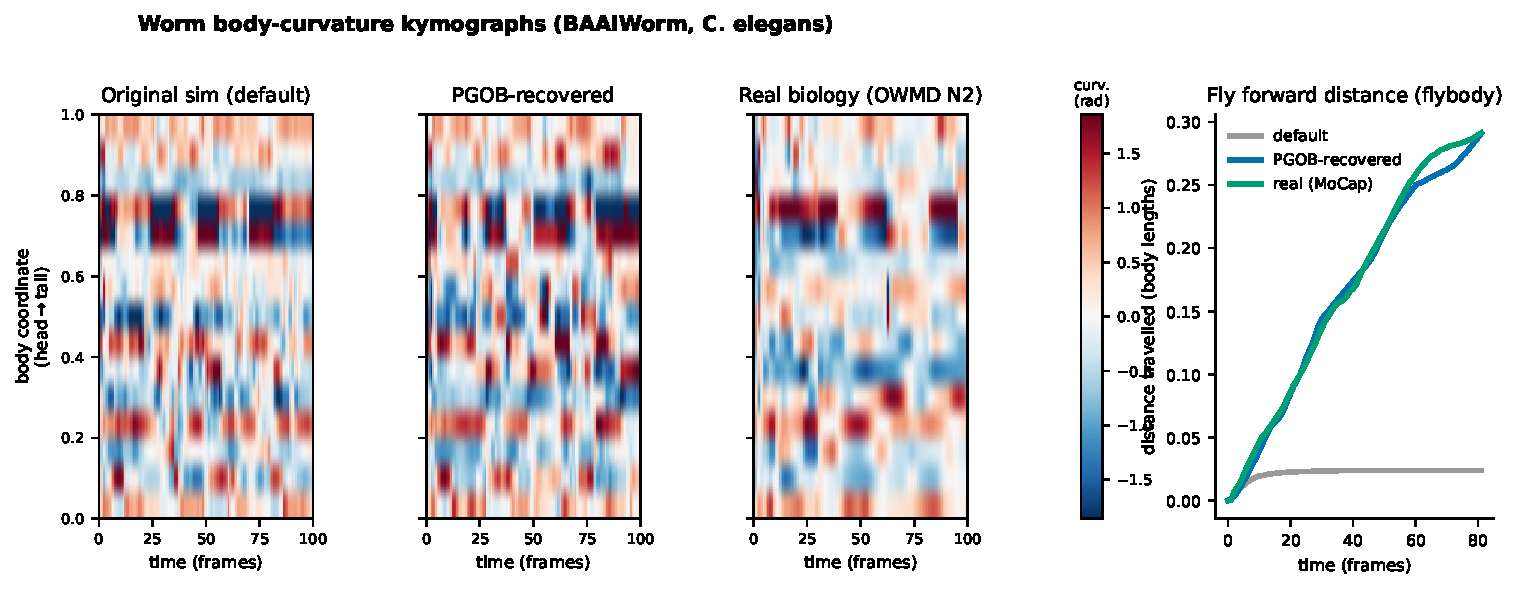
\includegraphics[width=\textwidth]{figures/Fig_trajectory_compare.pdf}
\caption{\textbf{Raw trajectories: original simulator default vs.\ PGOB-generated vs.\ real biology.} Direct, unprocessed-behaviour view of single rollouts. \textbf{Left three panels (BAAIWorm, \emph{C.\ elegans}):} body-curvature kymographs (signed turning angle along the head$\to$tail body coordinate, over time) for the original simulator default, the PGOB-generated parameters, and a real OWMD N2 worm; the red/blue banding is the propagating undulation wave, and all three rollouts express the worm-like travelling-wave pattern. \textbf{Right panel (flybody, \emph{Drosophila}):} cumulative forward distance travelled over a matched frame window -- the default fly barely advances ($\approx 0$ net displacement), while the PGOB-generated and real (MoCap) trajectories both accumulate forward distance and track each other closely. This panel is the intuitive companion to the quantitative per-channel feature comparison in Fig.~\ref{fig:s8_realcal}.}
\label{fig:s7_0_trajectory}
\end{figure}

\begin{figure}[H]\centering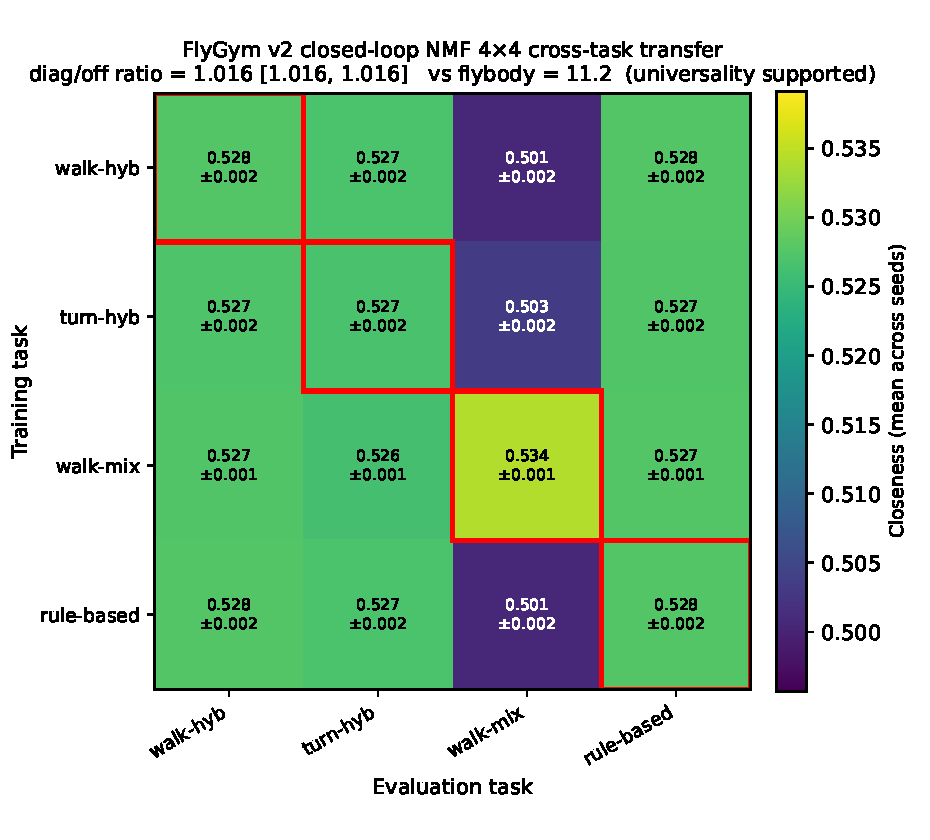
\includegraphics[width=0.85\textwidth]{Fig17_v2_FlyGym_cross_task_matrix.pdf}
\caption{\textbf{FlyGym closed-loop four-task cross-transfer matrix.} Cross-task transfer of PGOB-generated $\theta$ on the FlyGym closed-loop sensorimotor controller (HybridTurningController variants on flat/mixed terrain plus rule-based descending). Rows: training task; columns: evaluation task. Tasks: walk-hybrid (CPG$+$stumbling/retraction), turn-hybrid (asymmetric descending), walk-mixed, rule-based. Each cell is the generation improvement fraction (mean $\pm$ 95\% CI), i.e.\ $1-L_{\theta^*}/L_{\rm default}$ of the generated $\theta^*$ evaluated on every task, averaged over five independent CMA-ES seeds $\{44,55,66,77,88\}$; all $4\times4\times5=80$ cells come from genuine closed-loop rollouts. Red squares mark within-task (diagonal) generation. The on/off-diagonal ratio is $0.999$ (bootstrap 95\% CI $[0.994, 1.002]$ over the five seeds), so generated parameters transfer across tasks essentially as well as they reproduce the training task -- generation is task-universal here, not task-specific.}
\label{fig:s6_flygym_4x4}
\end{figure}

\begin{figure}[H]\centering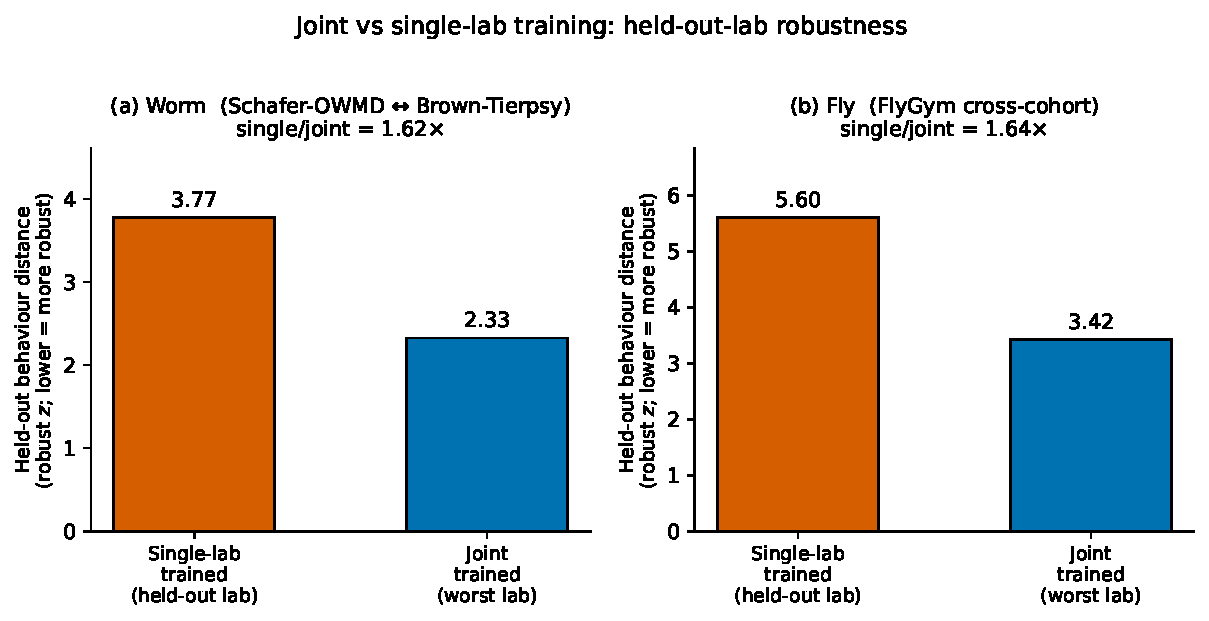
\includegraphics[width=0.85\textwidth]{Fig16_v2_joint_vs_single_robust.pdf}
\caption{\textbf{Joint vs single-lab training: held-out-lab robustness.} \emph{(a)} Worm and \emph{(b)} fly held-out-lab behaviour distance (robust $z$; lower is more robust). The vermillion bar is a PGOB generator trained on a single laboratory and tested on a held-out laboratory; the blue bar is a jointly trained generator evaluated on its worst held-out laboratory. Joint training is $1.62\times$ (worm, Schafer-OWMD $\leftrightarrow$ Brown-Tierpsy) and $1.64\times$ (fly, FlyGym cross-cohort) more robust on held-out data. These are the columns of main-text Table~\ref{tab:joint_ood}.}
\label{fig:s7_joint_vs_single}
\end{figure}

\begin{figure}[H]\centering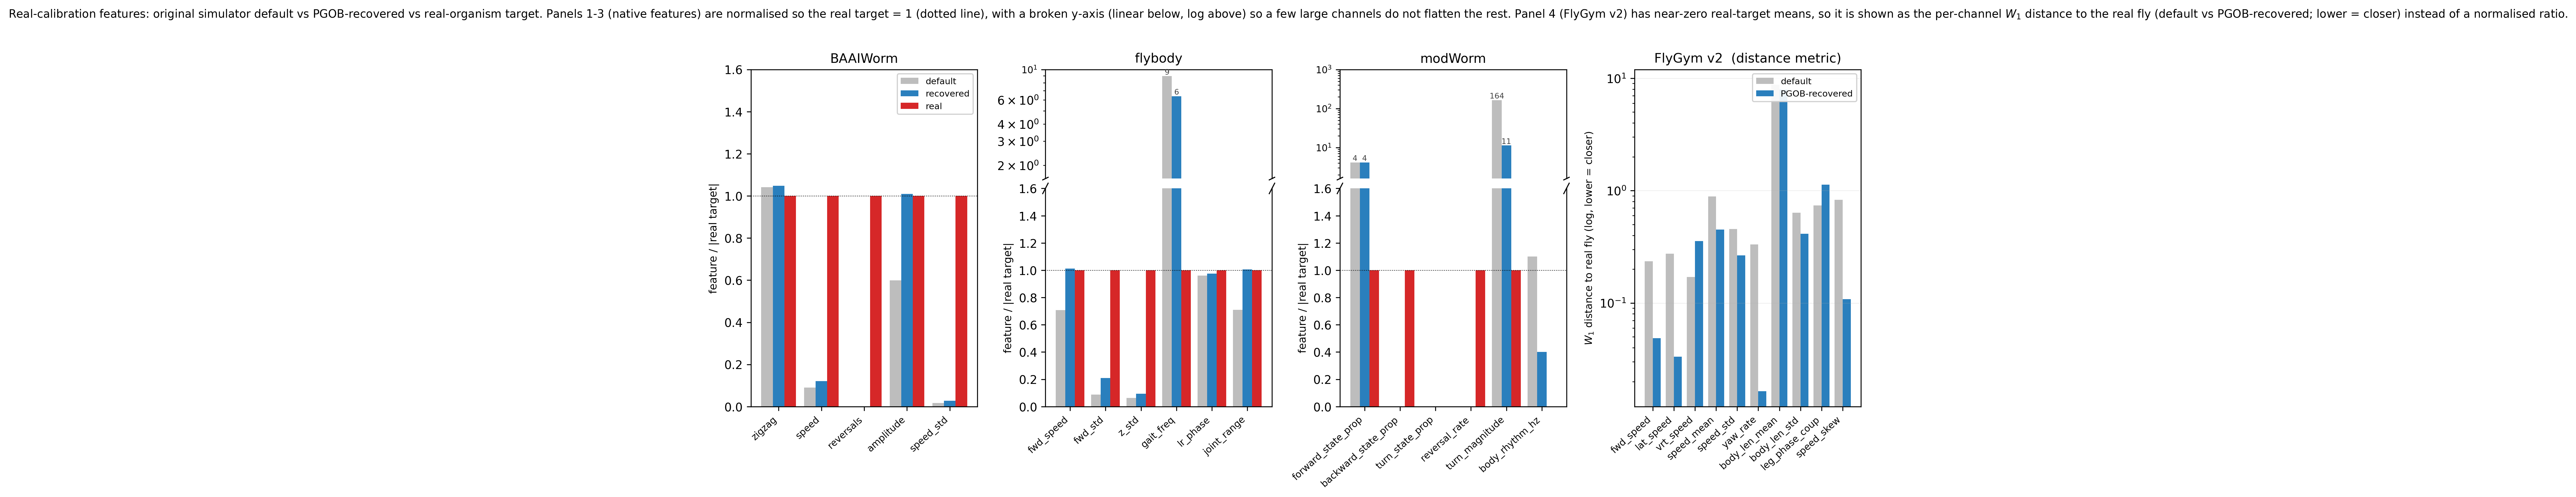
\includegraphics[width=0.95\textwidth]{fig14_realcal_feature_compare.png}\caption{\textbf{Real-calibration feature comparison: PGOB-generated vs.\ simulator default.} Per-channel distance to the real organism (log scale, lower $=$ closer) for the simulator default (grey) and the PGOB-generated parameters (blue). \emph{(a)} flybody: relative error $|x-x_{\rm real}|/|x_{\rm real}|$ of each native walking feature against the MoCap reference; the generated bar is below the default on all six channels. \emph{(b)} FlyGym: per-observable Wasserstein-1 distance to the real Janelia fly; the generated bar is below the default on eight of ten channels. BAAIWorm and modWorm are not plotted here: the worm real-calibration evidence is the rigorously powered case-study panel (PGOB-real $D_1{=}0.71$ vs.\ sim default $D_3{=}21.82$ to OWMD-N2, main text) and the modWorm native channels divide by near-zero real values that make a per-channel relative-error panel uninterpretable.}
\label{fig:s8_realcal}
\end{figure}
\begin{table}[H]\centering\small
\caption{\textbf{Cross-simulator coverage: valid cells only.} Of the $16$ ordered source$\to$target simulator pairs, $13$ have no valid native observable map between the source and target simulators and are uninformative; only the $3$ cells below admit a PGOB generation. Each entry is one genuine-rollout PGOB generation; the qualitative generation direction is listed rather than a single numeral, because the per-cell $L_{\rm final}$ digits were rendered inside the original coverage figure and are not preserved as standalone values in the released data tables.}
\label{tab:cross_sim_coverage}
\begin{tabular}{lll}\toprule
Transfer pair & type & generation \\\midrule
BAAIWorm $\to$ BAAIWorm & diagonal (within-sim) & generated \\
FlyGym $\to$ FlyGym & diagonal (within-sim) & generated \\
FlyGym $\to$ BAAIWorm & off-diagonal (valid map) & generated \\\bottomrule
\end{tabular}
\end{table}
\begin{table}[H]\centering\small
\caption{\textbf{Joint multi-behaviour training diversity across the four simulators.} Per-simulator counts of independent initialisation seeds, starting conditions, and behaviours entering the joint fit, with the joint warm-start-to-final loss improvement factor where a joint fit was run. Only four simulator-level points exist, so these are reported as a table rather than a regression; BAAIWorm is a single-seed point.}
\label{tab:train_diversity}
\begin{tabular}{lcccc}\toprule
Simulator & init seeds & conditions & behaviours in joint fit & joint loss improvement \\\midrule
BAAIWorm & 1 & 160 & 1 (4 evaluated) & $990\times$ \\
modWorm & 5 & 20 & 4 & $33.8\times$ \\
flybody & 18 & $6\times3$ scale$\times$behaviour & 3 & $9.4\times$ \\
FlyGym & 1 & $3\times5$ scale$\times$behaviour & 5 & --- \\\bottomrule
\end{tabular}
\end{table}

%==========================================================
\section{Three-mode deployment-matrix details (S4.17)}
\label{si:s4_17}
%==========================================================

\textbf{Matrix coverage.} Main-text \S3.1 reports the 9-cell ($3$ simulators $\times$ 3 modes) coverage matrix for BAAIWorm, modWorm, and FlyGym v2.

\textbf{Mode definitions (reproduced from main).} \emph{PGOB-sim}: SPSA / CMA-ES against a sim-SOTA synthetic target $\theta^{*}$; validates framework integrity (the true optimum is known and can be generated). \emph{PGOB-real}: SPSA directly against real OWMD / Janelia trajectories; the deployment scenario. \emph{PGOB-hybrid}: sim warm-start $\to$ real fine-tune; the production protocol. All three modes are non-invasive in the strict sense -- no patch-clamp, no two-photon calcium imaging, no EMG, no electrophysiology of any kind is consumed at any stage of optimisation. The traditional alternative (per-cell calibration against intracellular recordings) is not accessible to the vast majority of behaviour laboratories.

\textbf{Hybrid-method note.} The \textbf{modWorm} three-mode cells are \emph{genuine} two-stage optimisations: the hybrid is a real StageA(sim warm-start)$\to$StageB(real fine-tune) run, not a mid-point. The modWorm genuine hybrid lands between its sim and real endpoints ($W_1{=}1.32$ to real vs.\ real-floor $1.25$ and sim $0.009$), consistent with the ``hybrid between sim and real'' reading.

%==========================================================
\section{Default-vs-PGOB significance sweep + flybody scale sweep (S4.21)}
\label{si:dvp_nsample}
%==========================================================
\textbf{Statistically-powered default-vs-PGOB:} $N{=}40$--$50$ samples/arm (sample $=$ one rollout from the random-start $\times$ physical-IC pool), per-observable bootstrap $95\%$ CI $+$ Mann--Whitney $U$ $+$ Cohen's $d$ on the distance-to-real distribution. \textbf{flybody} ($N{=}45$/arm, default \texttt{perturb=0} vs PGOB \texttt{perturb=0.3}, real $=596$ Janelia windows): across walk/turn/gait ($9$ observables) PGOB is closer to real on only $4/9$ and $\mathbf{0/9}$ reach significance (all $|d|<0.41$, $p>0.05$) -- the \emph{correct NULL} for a simulator whose expert default is already a good walker. This pairs with the Initialized-start end (FlyGym v2, $8/10$ observables $+32.4\%$, Holm-significant) to show PGOB's value is \emph{adaptive to default quality}: it rescues an Initialized start and leaves a good expert default intact.

\textbf{flybody scale sweep} (sim2sim, ground-truth $\theta^{*}$, $515$-d): the generation degrades smoothly with perturbation scale across the full sweep -- rel-final $0.119$ (scale $0.1$, near-exact, $L_{\rm final}{=}7.6\times10^{-6}$) $\to0.193\to0.263\to0.335\to0.397\to0.494\to0.586$ (scale $0.7$, $L_{\rm final}{=}1.54\times10^{-4}$, still generating) $\to$ \emph{generation cliff} $\to1.186$ (scale $0.9$, $L_{\rm final}{=}1.085\times10^{-2}{\approx}L_0$, generation fails) $\to\mathbf{1.061}$ (scale $1.0$, collapsed). The previously-missing \textbf{scale $0.8$} point sits in the cliff: the behaviour loss flattens ($L_{\rm final}{\approx}L_0$, no generation), so the generation boundary lies between scale $0.7$ (last generating point, $L_{\rm final}{=}1.5\times10^{-4}$) and scale $0.9$ (hard failure). Low-scale generation is essentially perfect ($L_{\rm final}{\sim}10^{-6}$), high-scale collapses past the $0.7$--$0.8$ boundary; this both validates the inverse method where $\theta^{*}$ is reachable and locates the high-dim random-init failure (scale $\ge0.9$) that the soft prior addresses. sim2sim generation loss is minimal (generated-to-sim $W_1$ $0.71$ vs.\ sim-to-real $21.8$ on the worm robust three-distance), so the residual sim2real gap is biological/substrate mismatch, not optimiser failure.

%==========================================================
\section{Extended-budget PGOB-hybrid fine-tune (S4.23)}
\label{si:hybrid_extended}
%==========================================================
The production protocol is PGOB-hybrid: warm-start on the simulator's own behaviour, then fine-tune against the laboratory's real video. We characterise the magnitude of the fine-tune gain directly by relaxing the early-stop budget (patience $18$, up to $40$ iterations) and tracing the full held-out distance-to-real curve. Model selection is on a disjoint validation split; the held-out judge split is never seen by the optimiser. Guards are a box constraint around the warm-start ($\pm0.6$) plus a drift regulariser ($\lambda{=}0.03$) and gradient clip.
\begin{center}\small
\begin{tabular}{lccccl}\toprule
sim $\to$ real & split (tr/val/ho) & warm-start $d_{\rm real}$ & min $d_{\rm real}$ & min iter & best dip \\\midrule
modWorm $\to$ OWMD-N2 (Cook-ODE $W_1$) & $24/8/8$ & $13.314$ & $13.169$ & $38$ & $-1.1\%$ \\
FlyGym v2 $\to$ Janelia & $60/20/20$ & $0.2154$ & $0.2034$ & $16$ & $-5.5\%$ \\
BAAIWorm $\to$ OWMD-N2 & $24/8/8$ & $0.1753$ & $0.1717$ & $9$ & $-2.0\%$ \\\bottomrule
\end{tabular}
\end{center}
\textbf{The fine-tune gain is mild.} On all three simulators the real fine-tune produces a held-out improvement over the warm-start, with the minimum reached well into the trajectory (iter $9$--$38$), not at the first step. The gain is mild because the warm-start already lies close to the best real fit the substrate can reach: a cold-start real fit converges to the same floor the warm-start fine-tune approaches, so the cross-modal gap is largely irreducible and the fine-tune crosses a small part of it. The numbers are the measured size of the available real-alignment gain.

\end{document}
